\chapter{Eulerian Domain: Finite Element Method}

	\lsymb[f]{$\mathcal{T}_h$}{Finite Element mesh}{-}{th}		
	\lsymb[f]{$T$}{Cell of Finite Element mesh}{-}{t}			
	
	\lsymb[f]{$v$}{Test function}{-}{v}				
	\lsymb[f]{$V$}{Trial vector function space}{-}{vte}				
	\lsymb[f]{$\hat{V}$}{Test vector function space}{-}{vtr}					
	\gsymb[f]{$\Omega$}{Fluid domain}{-}{x}	
	\gsymb[f]{$\Omega_E$}{Eulerian fluid domain}{-}{xe}	
	\gsymb[f]{$\Omega_L$}{Lagrangian fluid domain}{-}{xl}	
	\gsymb[f]{$\partial \Omega$}{Boundary of the domain $\Omega$}{-}{xdd}	

%------------------------------------------------------------------------------------------------------
%------------------------------------------------------------------------------------------------------
%------------------------------------------------------------------------------------------------------
%\section{Purpose of eulerian domain}
Standard \printAcron{Computation Fluid Dynamics}{CFD} method discretizes the fluid into smaller regions, known as grids, and solves the set of Navier-Stokes equations in this region. This type of formulation is referred to as Eulerian method as we are evaluating the change of flow property in a given volume.

For the hybrid method, we use the Navier-Stokes grid formulation in the near-body region. The advantage of using the Eulerian method at this region is that it is much more efficient in resolving the boundary layer than the typical Vortex Particle Method. We can directly enforce the wall boundary condition at the wall boundary of the Eulerian domain, solving the problem of vorticity generation from a body. In the hybrid coupling strategy, we will interpolate this newly resolved near-wall solution on to the Lagrangian domain, where the vortex blobs will efficiently evolve the particles from the Lagrangian frame point.

The various approaches to solve the fluid dynamics problem from a Eulerian reference frame. \indexAcron{Finite Volume Method }{FVM}, \indexAcron{Finite Difference Method}{FDM}, and \indexAcron{Finite Element Method}{FEM} are the common choice for solving the Navier-Stokes problem and differ by the way they approach to solve the problem. FVM divides the domain into volumes where it enforces the conservation of mass and momentum in each sub-domains. FDM divides the domain into nodes and use local Taylor expansions to approximate the partial differential equations. FEM divides the domain into elements and solves the problem using variational calculus. So, in the end, the choice of Eulerian method does not have a direct impact on the coupling with the Lagrangian method. 

We have decided to use the FEM packages provided by the \texttt{FEniCS} project as they have be already implemented efficient, multi-threaded algorithms for solving differential equation and provide extensive features for future developments such as adaptive mesh refinement, fluid-structure interaction, and efficient computation of turbulence.

\section{Introduction to Finite Element Method}

\printAcron{Finite Element Method}{FEM} is numerical method to solve for the solution of a given differential equation. It is solved by describing it as a variation problem, and by minimizing the error we can reach a approximate solution for the boundary value problem \cite{Brenner2008}. So, the FEM approximates the unknown variables and converts the partial differential equations to algebraic equations. It was traditionally used for solid mechanics, for the analysis of aircraft structures \cite{Rao2005}, but have since then used to solve the Navier-Stokes fluid dynamics problems \cite{Guermond2006} \cite{Johnston2004} \cite{Guermond2003}.

\subsection*{Finite element discretization}

Finite Element solves by dividing the domain of interest into small, simple regions known as ``finite elements". These ``elements" are connected at the joints and are called nodes or nodal points. We use these sets of node and elements to represent the actual variation in the field (such as displacement, velocity, pressure or temperature) using simple functions, known as basis functions. Therefore, we have transformed a domain of infinite \indexAcron{Degrees of Freedom}{DOF} to a finite number of DOFs. We combine this set of equations of element equations into a global system of equations to solve for the final problem.

	\begin{figure}[b]
	\centering
	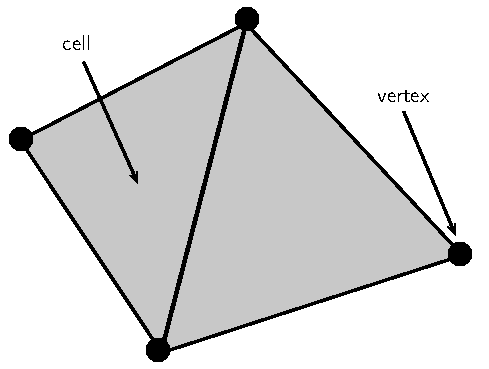
\includegraphics[width=0.4\linewidth]{./figures/eulerian/finiteElementDefinitions.pdf}
	\caption{A two-dimensional Finite Element geometry. The cell represents the area of the element, and vertices are the edge of the cell.}
	\label{fig:finiteElementDefinitions}
	\end{figure}

The discretization of a 2D domain can be observed in figure \ref{fig:finiteElementDefinitions}. The figures shows two connect finite elements. The cells represent the area of the element, and vertices of the cell are the node of the finite element. Therefore, we have divide the domain $\Omega$ into finite sets of cells $\mathcal{T}_h = \{T\}$ and together these cells make the mesh of the Eulerian domain. In 2D, the cells are made of simple geometrical shapes such as triangles, quadrilaterals, and tetrahedrals. There are two approaches to discretize the domain: structured and unstructured mesh. The structured mesh have cells that are of similar shape, such as rectangles and is the simplest approach in discretizing the mesh. The advantage of such discretization is that it has simple data structure and and can perform efficient computation. The downside is that the mesh quality deterioates ws the complexity of the domain increases. The common strategy of discretizing the domain for finite element method is to use an unstructured mesh, figure \ref{fig:cylinderFiniteElementDiscretization}. Even though this mesh data structure is complex, the advantage is that the mesh quality does not deteriorate with the domain complexity.

There are several algorithms for mesh generation. The standard approach is to employ the Delaunay triangulation method derived from the Voronoi diagram concept \cite{Carey1997}. This divides the domain into arbitrary number of triangles, figure \ref{fig:cylinderFiniteElementDiscretization}. This type of mesh generation allows us to connect shapes of different types in a simple manner. Furthermore, the triangulation method be controlled by predefining the boundary edges.

\begin{figure}[t]
        \centering
        \begin{subfigure}[b]{0.5\textwidth}
                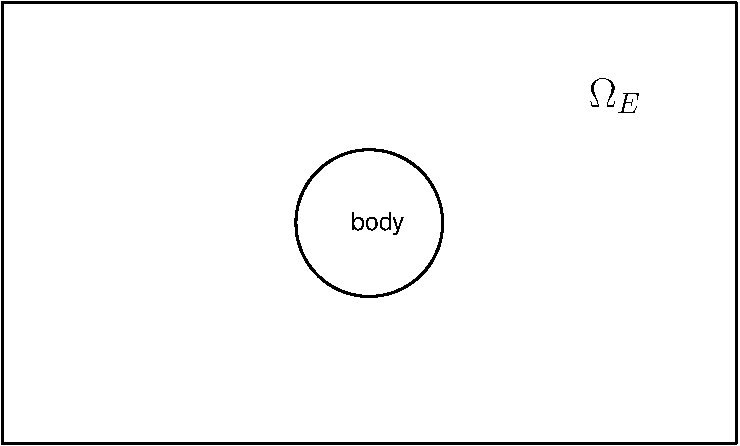
\includegraphics[width=\textwidth]{figures/eulerian/cylinderPreDelauney-crop.pdf}
                \caption{Fluid domain $\Omega_E$ around the cylinder}
                \label{fig:cylinderPreDelauney}
        \end{subfigure}%
        ~ %add desired spacing between images, e. g. ~, \quad, \qquad etc.
          %(or a blank line to force the subfigure onto a new line)
        \begin{subfigure}[b]{0.5\textwidth}
                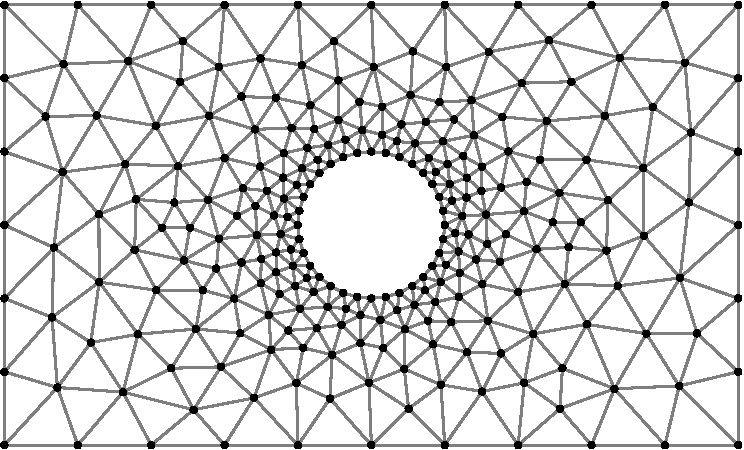
\includegraphics[width=\textwidth]{figures/eulerian/cylinderDelauney-crop.pdf}
                \caption{Delaunay triangulation of the fluid}
                \label{fig:cylinderDelauney}
        \end{subfigure}
        \caption{Delaunay triangulation of the fluid around a cylinder resulting in unstructured mesh with controllable cell sizes.}
        \label{fig:cylinderFiniteElementDiscretization}
\end{figure}	

\subsection*{Finite element function and function space}

When the domain $\Omega$ is divided into cells $T$, we can define the function and the function space of the Finite element problem. For each cell, a local function space $\mathcal{V}$ can be defined to collectively construct the global function space $V$.

There are several numbers of Finite Element families. 

\todo{Summary of libraries}
\subsection*{Variational problem}
\label{subsec:variationalProblem}

To solve a basic problem such as a Poisson equation numerically, we need to convert it into a variational problem. The methodology is followed from the \texttt{FEniCS} tutorial provide by Langtangen \cite{Langtangen2012}. A 1D Poisson problem is given as,

	\begin{subequations}
	\begin{align*}
	- \nabla^2 u(x) &= f(x), \qquad x\ \mathrm{in}\ \Omega,\\
	u(x) &= u_0(x), \qquad x\ \mathrm{on}\ \partial\Omega.
	\end{align*}
	\label{eq:poissonEq}
	\end{subequations}
	
We can transform equation \ref{eq:poissonEq} into the variational form by multiplying with a test function $v$, and integrating it over the domain $\Omega$,


	\begin{equation}
	- \int_{\Omega} \left(\nabla^2 u\right)v\ \mathrm{d}x= \int_{\Omega} fv\ \mathrm{d}x.
	\label{eq:poissonEqVariationFormA}
	\end{equation}

The function $u$ in variational form, equation \ref{eq:poissonEqVariationFormA}, is known as the trial function and it is the solution that we are trying to approximate. The test function $v$ lies in the test function space $\hat{V}$ and our trial function $u$ lies on the function space $V$. When performing integration by parts, the test function $v$ is required to be zero at regions where $u$ is known. So, the additional terms cancel and we get,

	\begin{equation}
	- \int_{\Omega} \nabla u \nabla v\ \mathrm{d}x= \int_{\Omega} fv\ \mathrm{d}x \qquad \forall v \in \hat{V}
	\label{eq:poissonEqVariationFormB}
	\end{equation}

This form is referred to as the ``weak-form" of the original Poisson equation and is valid for all $v$ in the trial space $\hat{V}$. In order to solve this continuous problem numerically, we must discretize it first into discrete variational problem,

	\begin{equation}
	- \int_{\Omega} \nabla u_h \nabla v\ \mathrm{d}x= \int_{\Omega} fv\ \mathrm{d}x \qquad \forall v \in \hat{V}_h \subset \hat{V},
	\label{eq:poissonEqDiscreteVariational}
	\end{equation}

where $u_h$ is the discrete function in the discrete space $V_h$ which is a subset of $V$ and the discrete function space $\hat{V}_h$ is a subset of $\hat{V}$. A common choice for the function space is linear triangular element with three nodes, figure \ref{fig:finiteElementDefinitions}, where $\hat{V}_h$ and $V_h$ are described by the piecewise linear functions of the triangles and the functions of this function of the test space is zero at the boundary and the function of the trial space is equal to the boundary condition $u_0$.

The equation \ref{eq:poissonEqDiscreteVariational} can be summarized as follows,

	\begin{equation}
	a\left(u,v\right) = L(v),
	\label{eq:weakForm}
	\end{equation}

where $a\left(u,v\right) = - \int_{\Omega} \nabla u \nabla v\ \mathrm{d}x$, and $L(v)=\int_{\Omega}fv\ \mathrm{d}x$ and is referred to as bilinear and linear form, respectively. To solve for the discrete solution we substitute,
	
	\begin{equation}
	u = \sum_{j=1}^{N} U_j \phi_j,
	\label{eq:trialDiscrete}
	\end{equation}

a linear combination of the basis function $\phi_j$, spanning the function space $V$, into $a\left(u,v\right)$. The test function is linear combination of the basis function $\hat{\phi}_i$, spanning the test space $\hat{V}$, is defined as

	\begin{equation}
	v=\sum_{i=1}^{N} \hat{\phi}_i.
	\label{eq:testDiscrete}
	\end{equation}
	
The test function $v$ is taken to be zero at the boundary and one everywhere else. Substituting equation \ref{eq:trialDiscrete} and \ref{eq:testDiscrete} into equation \ref{eq:weakForm} gives,
	
	\begin{equation}
	\sum_{j=1}^N a(\phi,\hat{\phi}_i)\ U_j = L(\hat{\phi}_i).
	\end{equation}

Thus, we have to solve a linear system of equations given as,

	\begin{equation}
	\mathbf{A}U = b,
	\label{eq:linearSysOfEq}
	\end{equation}	
	
where $\mathbf{A}_{ij} = a(\phi_j,\hat{\phi}_i)$ is the coefficient matrix, and $b$ is the \printAcron{Right-Hand Side}{RHS} containing the knowns of the problem.
 	
%------------------------------------------------------------------------------------------------------
%------------------------------------------------------------------------------------------------------
%------------------------------------------------------------------------------------------------------
\section{Solving the Finite Element problem}

To solve this linear system of equations, equation \ref{eq:linearSysOfEq}, we use the \texttt{FEniCS} Project that has implemented a comprehensive library of finite elements, and high performance linear algebra. The \texttt{DOLFIN} library from the \texttt{FEniCS} Project was used to define the Eulerian domain of the hybrid coupling scheme.

In order to generate the mesh of the fluid domain, we used \texttt{GMSH}, a three-dimensional finite element mesh generator which proves a fast, light and user-friendly meshing tools.

\subsection{Introduction to FEniCS Project}

	\begin{figure}[b]
	\centering
	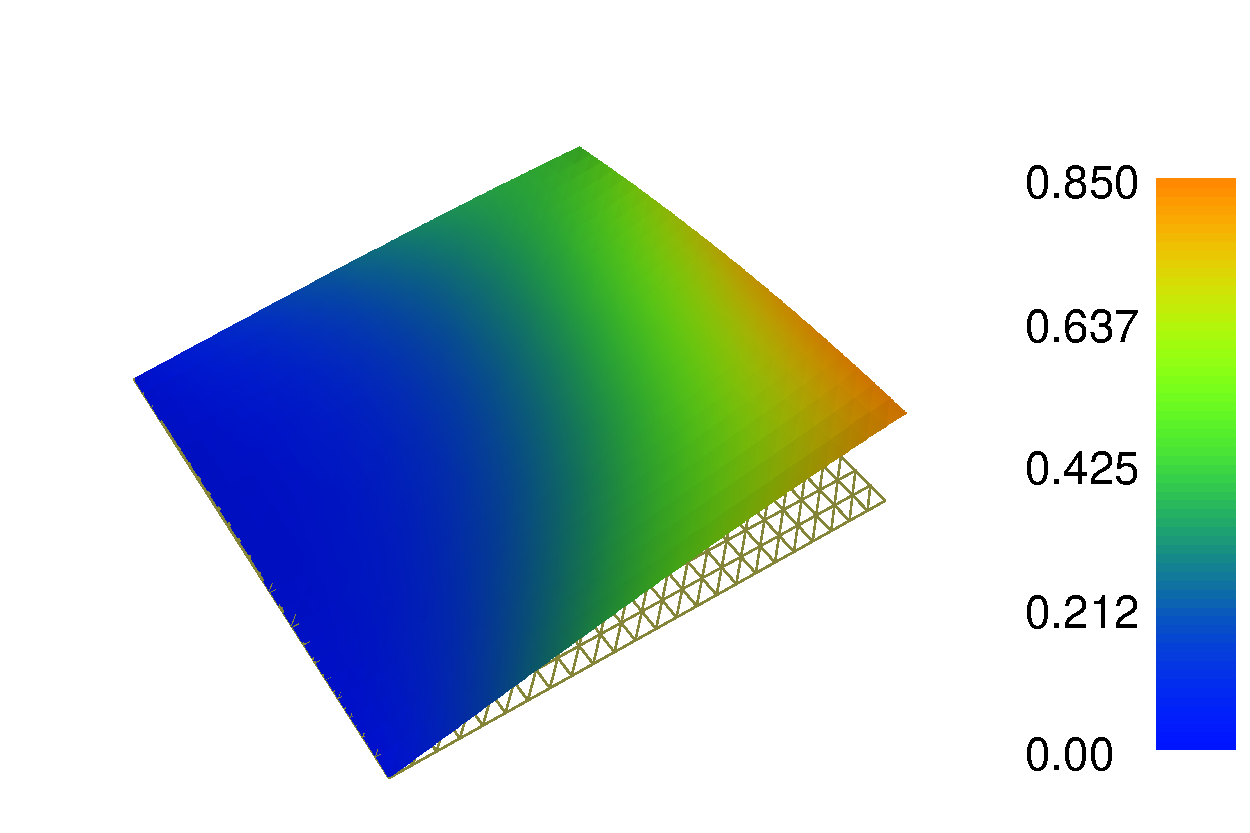
\includegraphics[width=0.5\linewidth]{./figures/eulerian/dolfinExampleFigure-rotated270.pdf}
	\caption{\texttt{DOLFIN} \texttt{VTK} plot of the Poisson solution, given by the problem, listing \ref{lst:pycode-poisson}.}
	\label{fig:dolfinExampleFigure}
	\end{figure}

The \texttt{FEniCS} Project is a collaborative work of various universities, that developed tools to automated Finite Element Methods for solving the solutions of differential equation \cite{FenicsAbout}. It was a project originated in 2003 with the research collaboration of University of Chicago and Chalmers University of Technology with Logg,  Mardal, and Wells \cite{Logg2012a}. Since then, it has been expanded to various institutes such as Royal Institute of Technology, Simula Research Laboratory, Univeristy of Cambridge, and Delf Universty of Technology.

The consists of various libraries such as \texttt{UFC}, \texttt{UFL}, \texttt{FIAT}, \texttt{Instant} and mainly \texttt{DOLFIN}. \texttt{DOLFIN} is the core library aimed at automating the solution of partial differential equations using finite element method \cite{Logg2011}. It uses automated code generation maintaining high level of mathematical expressions and internally providing efficient, multi-threaded performance using the \indexAcron{Message Passing Interface}{MPI}. It used built-in linear algebra backend such as \texttt{PETSc}, \texttt{Trilinos/Epectra}, \texttt{uBLAS}, and \texttt{MTL4}.

The Poisson problem,

	\begin{equation}
	-\nabla^2 u = f,
	\end{equation}

with $f=2$ and $u(x) = u_0(x) = \sin x \cdot \cos y$ on boundary $\partial \Omega$ can be automated using the \texttt{DOFLIN} library. The solution algorithm follows from section \ref{subsec:variationalProblem}. The ection \ref{subsec:variationalProblem} can be seen in listing \ref{lst:pycode-poisson}.

	\begin{listing}[p]
	\inputminted[fontseries=courier,obeytabs,fontsize=\footnotesize,mathescape,linenos,numbersep=5pt,frame=lines,framesep=2mm,xleftmargin=20mm,xrightmargin=20mm]{python}{figures/eulerian/dolfinExample.py}
	\caption{A complete program for solving the Poisson problem and plotting the solution. The Poisson problem is given as $-\nabla^2{u} = f$, where $u_0 = \sin{x}\cdot\cos{y}$ on the boundary and $f=2$. The code is written in python using \texttt{DOLFIN} 1.2 library}
	\label{lst:pycode-poisson}
	\end{listing}
	

\subsection{Mesh generation using GMSH}


%------------------------------------------------------------------------------------------------------
%------------------------------------------------------------------------------------------------------
%------------------------------------------------------------------------------------------------------
\section{Solving Incompressible Navier-Stokes Equations}

\subsection{Velocity-pressure formulation}

\subsection{Incremental pressure correction scheme}

\subsection{Determining the vorticity field}

\subsection{Determining the body forces}

\subsubsection*{Frictional Forces}

\subsubsection*{Pressure Forces}


\section{Validation of eulerian method}

%\subsection{Lamb-oseen vortex}

\subsection{Clercx-Bruneau dipole collison at $Re=625$}

\subsection{Impulsively started cylinder at $Re=550$}

\section{Summary}

